\documentclass{article}
\usepackage[utf8]{inputenc}
\usepackage[T1]{fontenc}
\usepackage{graphicx}
\usepackage{algorithm}
\usepackage{algpseudocode}

\usepackage{listings}
\usepackage{xcolor}
\usepackage[margin=2cm]{geometry}
\usepackage{float}

\usepackage{amssymb} %Ajoute des symboles mathématiques comme R, Z, forall, exists, etc....
\usepackage{amsmath}
\usepackage{amsthm}

\usepackage{enumitem}


\lstdefinestyle{monstyle}{
    backgroundcolor=\color{white},
    commentstyle=\color{gray},
    keywordstyle=\color{blue},
    numberstyle=\tiny\color{gray},
    basicstyle=\ttfamily\small,
    breaklines=true,
    numbers=left,
    numbersep=5pt,
    frame=single,
}
\lstset{style=monstyle}


\usepackage{soul} % IMPORTANT : POUR SURLIGNER AVEC \hl en fin de ligne 
\usepackage{xcolor}


\title{\sethlcolor{pink!30}\hl{\textbf{Fichier de révisions: Environnement de travail -- LaTeX - Beamer - TikZ}}}
\author{Derrez Lorenzo}

\begin{document}
\maketitle

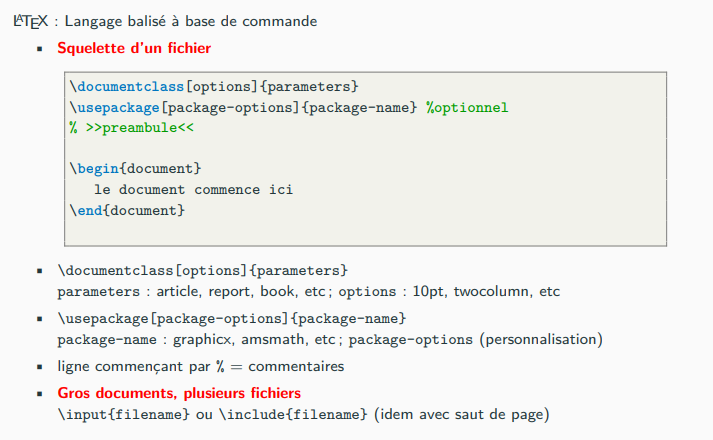
\includegraphics[width=0.80\textwidth]{structure_base.png}
\\
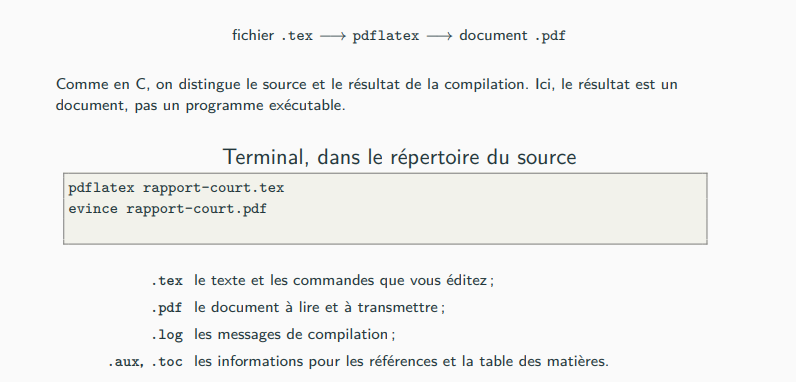
\includegraphics[width=0.80\textwidth]{term_comp_latex.png}

\section*{\hl{\textbf{Environnement}}}

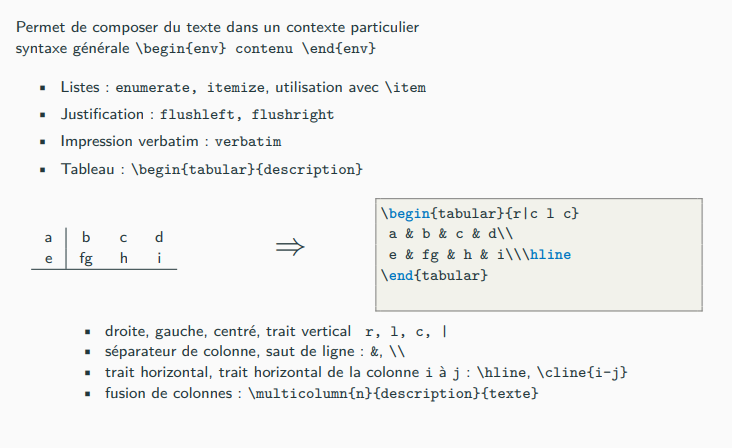
\includegraphics[width=0.80\textwidth]{env_base.png}

\section*{\hl{\textbf{Flottans \& Inclusions de figure}}}

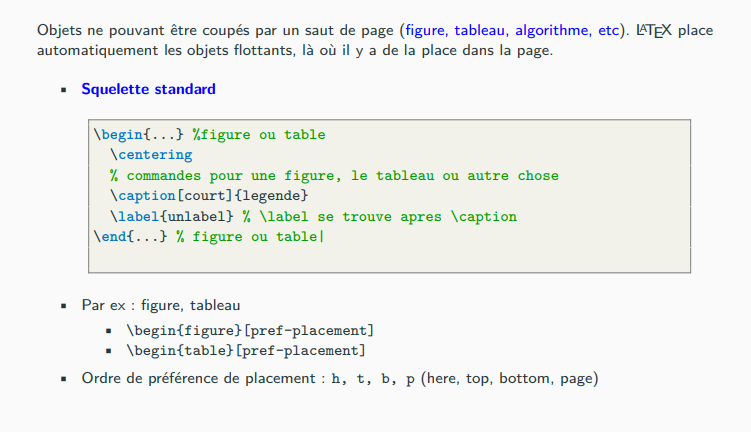
\includegraphics[width=0.50\textwidth]{squel_std_flottant.png}
\\
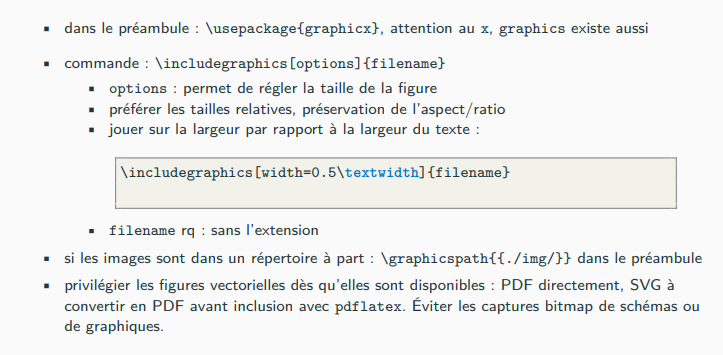
\includegraphics[width=0.50\textwidth]{incl_grapx.png}

\begin{itemize}
    \item \textbf{NE JAMAIS:} mettre une figure sans titre, sans référence dans le texte.
    \item \textbf{IMPORTANT:} un flottant (image, tableau,...) doit toujours: 
    \subitem comporter une légende explicative
    \subitem être cité, référencé dans le texte à l'aide de \text{"antislash\_label"}
    \subitem Le flottant fait partie de la phrase, on ne le cite pas entre parenthèse.
\end{itemize}

\section*{\hl{\textbf{AMS-LateX}}}

\begin{itemize}
    \item AMS $\implies$ collection d'extensions et de classes pour les saisies scientifiques/mathématiques
    \item usepackage amsmath, amssymb
\end{itemize}

\subsection*{Pour les équations:}

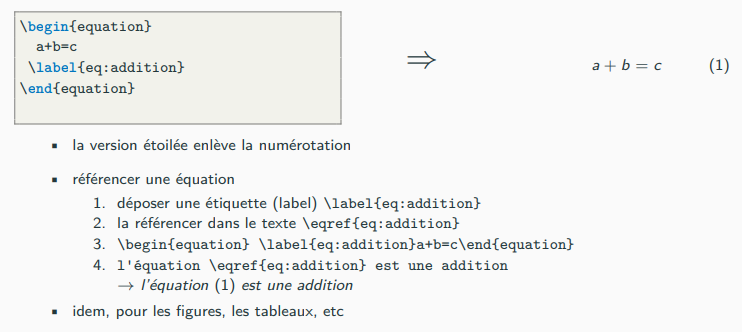
\includegraphics[width=0.50\textwidth]{struct_eq.png}

\subsection*{Pour les calculs \textbf{alignés}:}

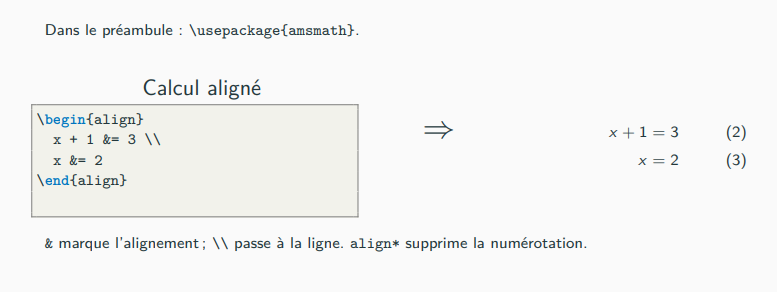
\includegraphics[width=0.50\textwidth]{align.png}

\subsection*{Pour les systèmes:}

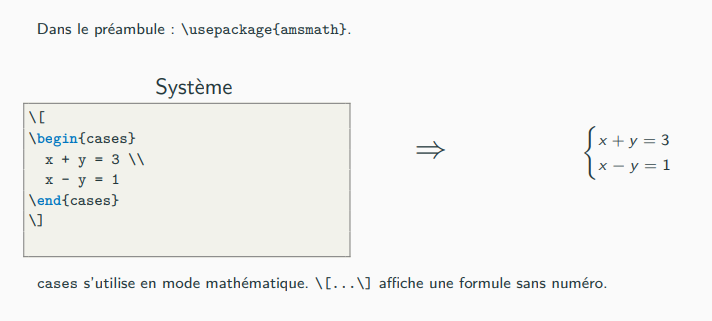
\includegraphics[width=0.50\textwidth]{syst.png}

\subsection*{Pour les algorithmes:}

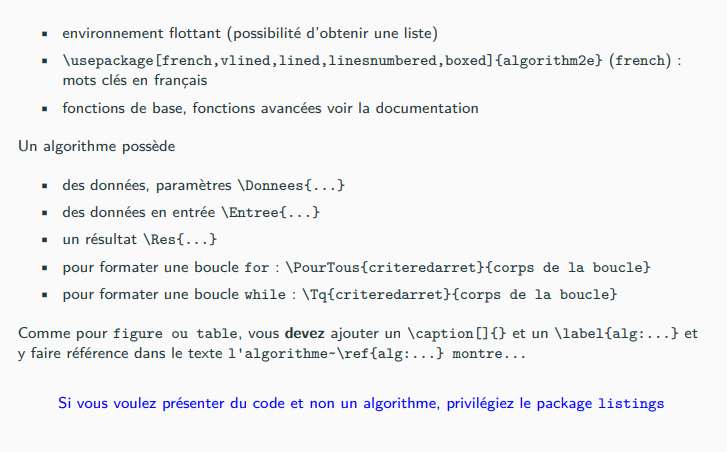
\includegraphics[width=0.50\textwidth]{algo1_notes.png}
\\
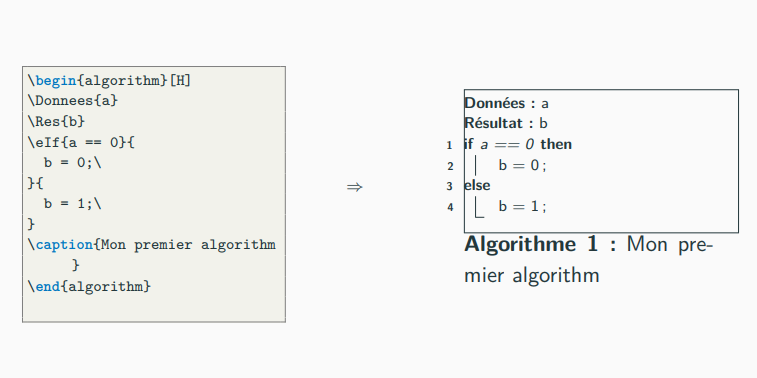
\includegraphics[width=0.50\textwidth]{algo2.png}

\textbf{Remarque Personnelle:} Je préfère utiliser les modules algorthm et algorithmic pour faire des algos. La mise en page est meilleure et plus lisible.

\section*{\hl{\textbf{Beamer}}}

\subsection*{Introduction}

\begin{itemize}
    \item classe de document au même titre que \textit{article, report, book}
    \item permet de concevoir des présentations en LateX
\end{itemize}

\textbf{Caractéristiques:}

\begin{itemize}
    \item accepte les commandes LateX
    \item pratique pour la structuration, les équations, etc
    \item permet de créer des animations
    \item pluralités de thèmes adaptés pour les présentations.
    \item thèmes conçus pour être très lisibles 
    \item thèmes hautement configurable
\end{itemize}

\subsection*{Structure de base:}

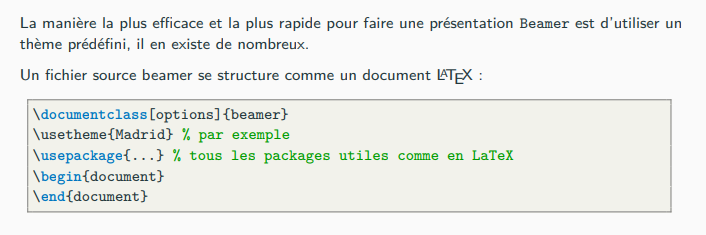
\includegraphics[width=0.80\textwidth]{struct_base_beamer.png}
\\
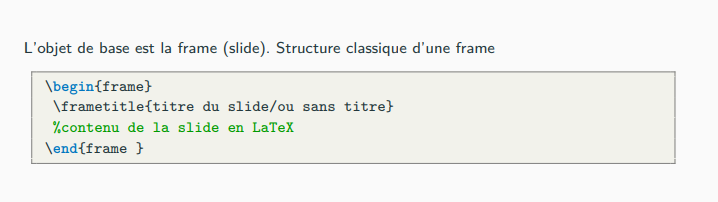
\includegraphics[width=0.80\textwidth]{frame.png}
\\
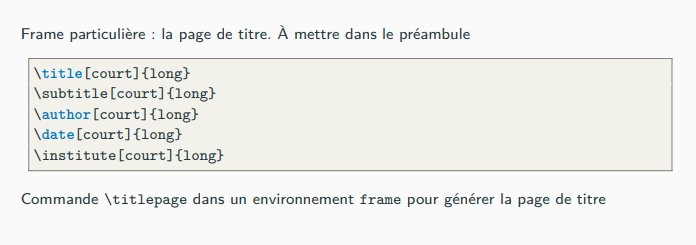
\includegraphics[width=0.80\textwidth]{frame_part.png}

\subsection*{Blocs \& Listes}

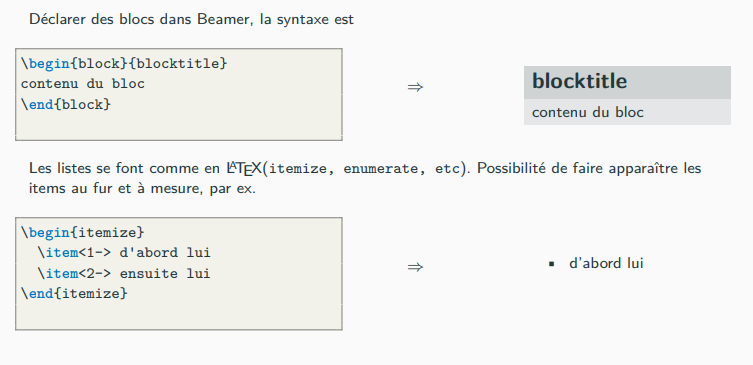
\includegraphics[width=0.80\textwidth]{block&title.png}
\\
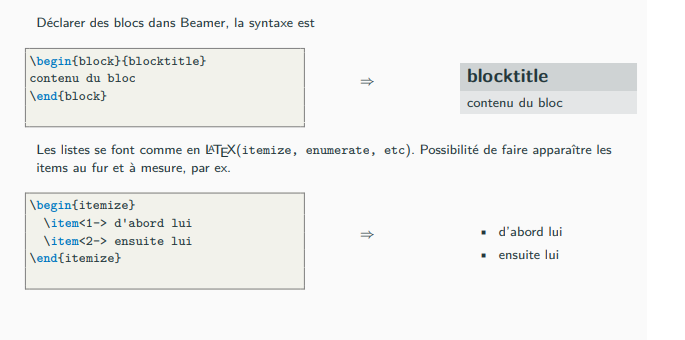
\includegraphics[width=0.80\textwidth]{block&titlev2.png}

\section*{\hl{\textbf{Règles pour les présentations orales:}}}

\begin{itemize}
    \item comporte \textbf{toujours}: une page de titre, un plan, une Introduction, le pourquoi de la présentation, une conclusion.
    \item chaque slide/diapo ne doit pas être trop chargée.
    \item doit être structurée et claire
    \item éviter de faire des animations de transitions.
    \item favorisé la sobriété et la clarté
    \item Environ 1 à 2 minutes par slide. 
    \item Favoriser des schémas ou des diagrammes (avec sources \& références)
\end{itemize}

\section*{\hl{\textbf{TikZ}}}

\begin{itemize}
    \item décrit des positions, des formes, des noeuds, et des liens. 
    \item La compilation $\implies$ un dessin vectoriel intégré au document.
    \item les textes et les formules utilisent les mêmes polices que le document.
    \item Utiles pour : 
    \subitem schéma, arbre, automate, $\ldots$
\end{itemize}

\subsection*{Utilisation TikZ de base:}

\begin{itemize}
    \item utiliser le package tikz 
    \item pour commencer un graphique: 
    \subitem begin tikzpicture et end tikzpicture
    \item chaque instruction doit se terminer par \textit{;}
\end{itemize}

\subsection*{Exemples d'utilisation de TikZ}

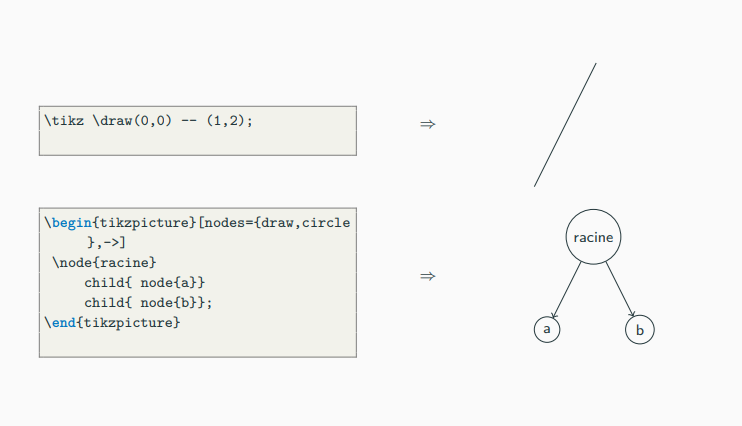
\includegraphics[width=0.80\textwidth]{tikz_ex1.png}
\\
\textbf{Pour nommer et relier des noeuds:}
\\
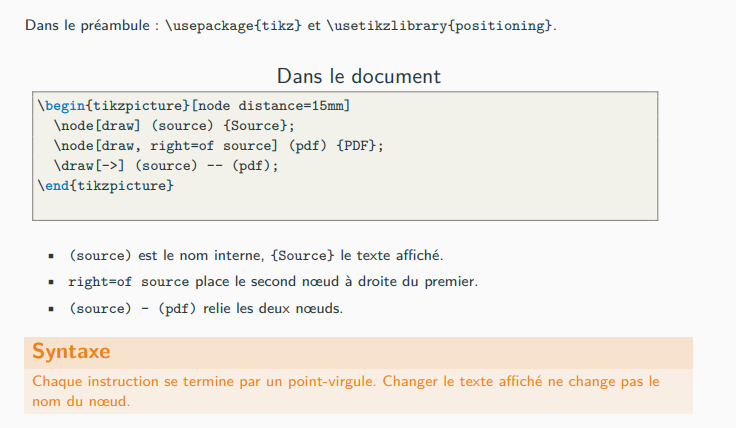
\includegraphics[width=0.80\textwidth]{nomm.png}

\subsection*{\textbf{Références LateX commandes:}}

\textbf{COMMANDE DISPO DANS LE DOCU DE COURS}

\end{document}